\section{Modules Explanation}

\subsection{\texttt{Add} Module}

\texttt{Add} module reads two signed $32$-bits integers as input, and outputs a signed $32$-bit integer, which is the sum of the two input integers.

\subsection{\texttt{ALU\_Control} Module}

\texttt{ALU\_Control} module reads the $12..14, 25..31$-th bits of the instruction, \texttt{ALUOp} as input, and outputs \texttt{ALUOp3}, which will be used by \texttt{ALU} later. The module uses \texttt{ALUOp} to determine if the instruction is addi, srai, noop, beq, or others, and then uses those $10$ bits of the instruction to determine what kind of instruction it is. The value of \texttt{ALUOp3} is as follow:\\
\texttt{0:and 1:xor 2:sll 3:add 4:sub 5:mul 6:srai}.

\subsection{\texttt{ALU} Module}

\texttt{ALU} module reads \texttt{a}, \texttt{b}, \texttt{op} as input, and outputs \texttt{c}. The module uses \texttt{ALUOp3} to determine which operation should be done to \texttt{a}, \texttt{b}, and then calculates the result as \texttt{c}.

\subsection{\texttt{Control} Module}

\texttt{Control} module reads the $0..6$-th of the instruction, \texttt{noop} as input, and outputs the six control signals: \texttt{RegWrite}, \texttt{MemtoReg}, \texttt{MemRead}, \texttt{Write}, \texttt{ALUOp}, \texttt{ALUSrc}, which are stored in \texttt{ctrl} in this order, and the signal \texttt{Branch\_o}. If the instruction is all $0$ or \texttt{noop} is true, then it outputs all control signals in $0$. Otherwise, it outputs the control signals in what is written in the slide.

\subsection{\texttt{ForwardingUnit} Module}

\texttt{ForwardingUnit} module reads \texttt{rs1} and \texttt{rs2} from \texttt{EX} stage, \texttt{RegWrite} and \texttt{Rd} from \texttt{MEM} and \texttt{WB} stages as input, and outputs \texttt{fa} (\texttt{Forwarding A}), \texttt{fb} (\texttt{Forwarding B}) using the rule in the spec.

\subsection{\texttt{HazardDetectionUnit} Module}

\texttt{HazardDetectionUnit} module reads \texttt{rs1} and \texttt{rs2} from \texttt{ID} stage, \texttt{rd} and \texttt{MemRead} from \texttt{EX} stage as input, and outputs \texttt{PCWrite}, \texttt{Stall\_o}, and \texttt{noop}. The hazard happens when \texttt{MemRead} is set to be true, and the register to be written is one of \texttt{rs1}, \texttt{rs2}. Therefore, \texttt{Stall\_o} and \texttt{noop} is set to be true when the above happens. Besides, the program counter needs to be changed when the operation is not \texttt{noop}, and therefore \texttt{PCWrite} is set to be true when \texttt{noop} is not true.

\subsection{\texttt{ImmGen} Module}

\texttt{ImmGen} module reads the instruction as input, and outputs the immediate storing in the instruction (which is \texttt{res}). It determines which instruction it is using \texttt{funct3} and \texttt{opcode}, and then outputs the correspond (signed extend) value of immediate using the form given in the spec.

\subsection{\texttt{MUX2} Module}

\texttt{MUX2} module reads $32$-bits $a_0, a_1$ and $1$-bit $sel$ as input, and outputs $a_{sel}$ as $b$.

\subsection{\texttt{MUX4} Module}

\texttt{MUX4} module reads $32$-bits $a_0, a_1, a_2, a_3$ and $2$-bits $sel$ as input, and outputs $a_{sel}$ as $b$.

\subsection{\texttt{IFID} Module}

\texttt{IFID} module reads clock signals, reset bit, next cycle PC, inst, \texttt{flush}, \texttt{stall} as input, and outputs the PC of the current cycle. This module changes its internal register \texttt{pc}, \texttt{inst} at the positive edge of the clock signal. When the reset bit is set, \texttt{pc}, \texttt{inst} are reset to $0$. Besides, if \texttt{flush} is set, it means that it must jump to another stage, which should flush its current inst. And if \texttt{stall} is set, then its internal register \texttt{pc}, \texttt{inst} won't be changed at the positive edge of the clock signal.

\subsection{\texttt{IDEX} Module}

\texttt{IDEX} module reads clock signals, reset bit, next cycle control signals (stored in \texttt{ctrli} in the order same as that in \texttt{Control} module), rs1, rs2, immediate, inst as input, and outputs the control signals, rs1, rs2, immediate, inst of the current cycle. Note that on the figure given in the spec, it only deals with \texttt{inst[7..11, 15..19, 20..24]}, but in my implementation, I deal with \texttt{inst[0..31]}. This module changes its internal register \texttt{ctrl}, \texttt{r1} (rs1), \texttt{r2} (rs2), \texttt{imm} (immediate), \texttt{inst} at the positive edge of the clock signal. When the reset bit is set, those registers are reset to $0$.

\subsection{\texttt{EXMEM} Module}

\texttt{IDEX} module reads clock signals, reset bit, next cycle control signals (stored in \texttt{ctrli} in the order \texttt{RegWrite}, \texttt{MemtoReg}, \texttt{MemRead}, \texttt{MemWrite}), ALU result, forward value of rs2, rd as input, and outputs the control signals, ALU result, forward value of rs2, rd of the current cycle. This module changes its internal register \texttt{ctrl}, \texttt{alu} (ALU result), \texttt{r2} (forward value of rs2), \texttt{inst} at the positive edge of the clock signal. When the reset bit is set, those registers are reset to $0$.

\subsection{\texttt{MEMWB} Module}

\texttt{MEMWB} module reads clock signals, reset bit, next cycle control signals (stored in \texttt{ctrli} in the order \texttt{RegWrite}, \texttt{MemtoReg}), ALU result, data read in memory, rd as input, and outputs the control signals, ALU result, data read in memory, rd of the current cycle. This module changes its internal register \texttt{ctrl}, \texttt{alu1} (ALU result), \texttt{alu2} (data read in memory), \texttt{rd} at the positive edge of the clock signal. When the reset bit is set, those registers are reset to $0$.

\subsection{\texttt{CPU} Module}

This module simulates the following circuit:\\
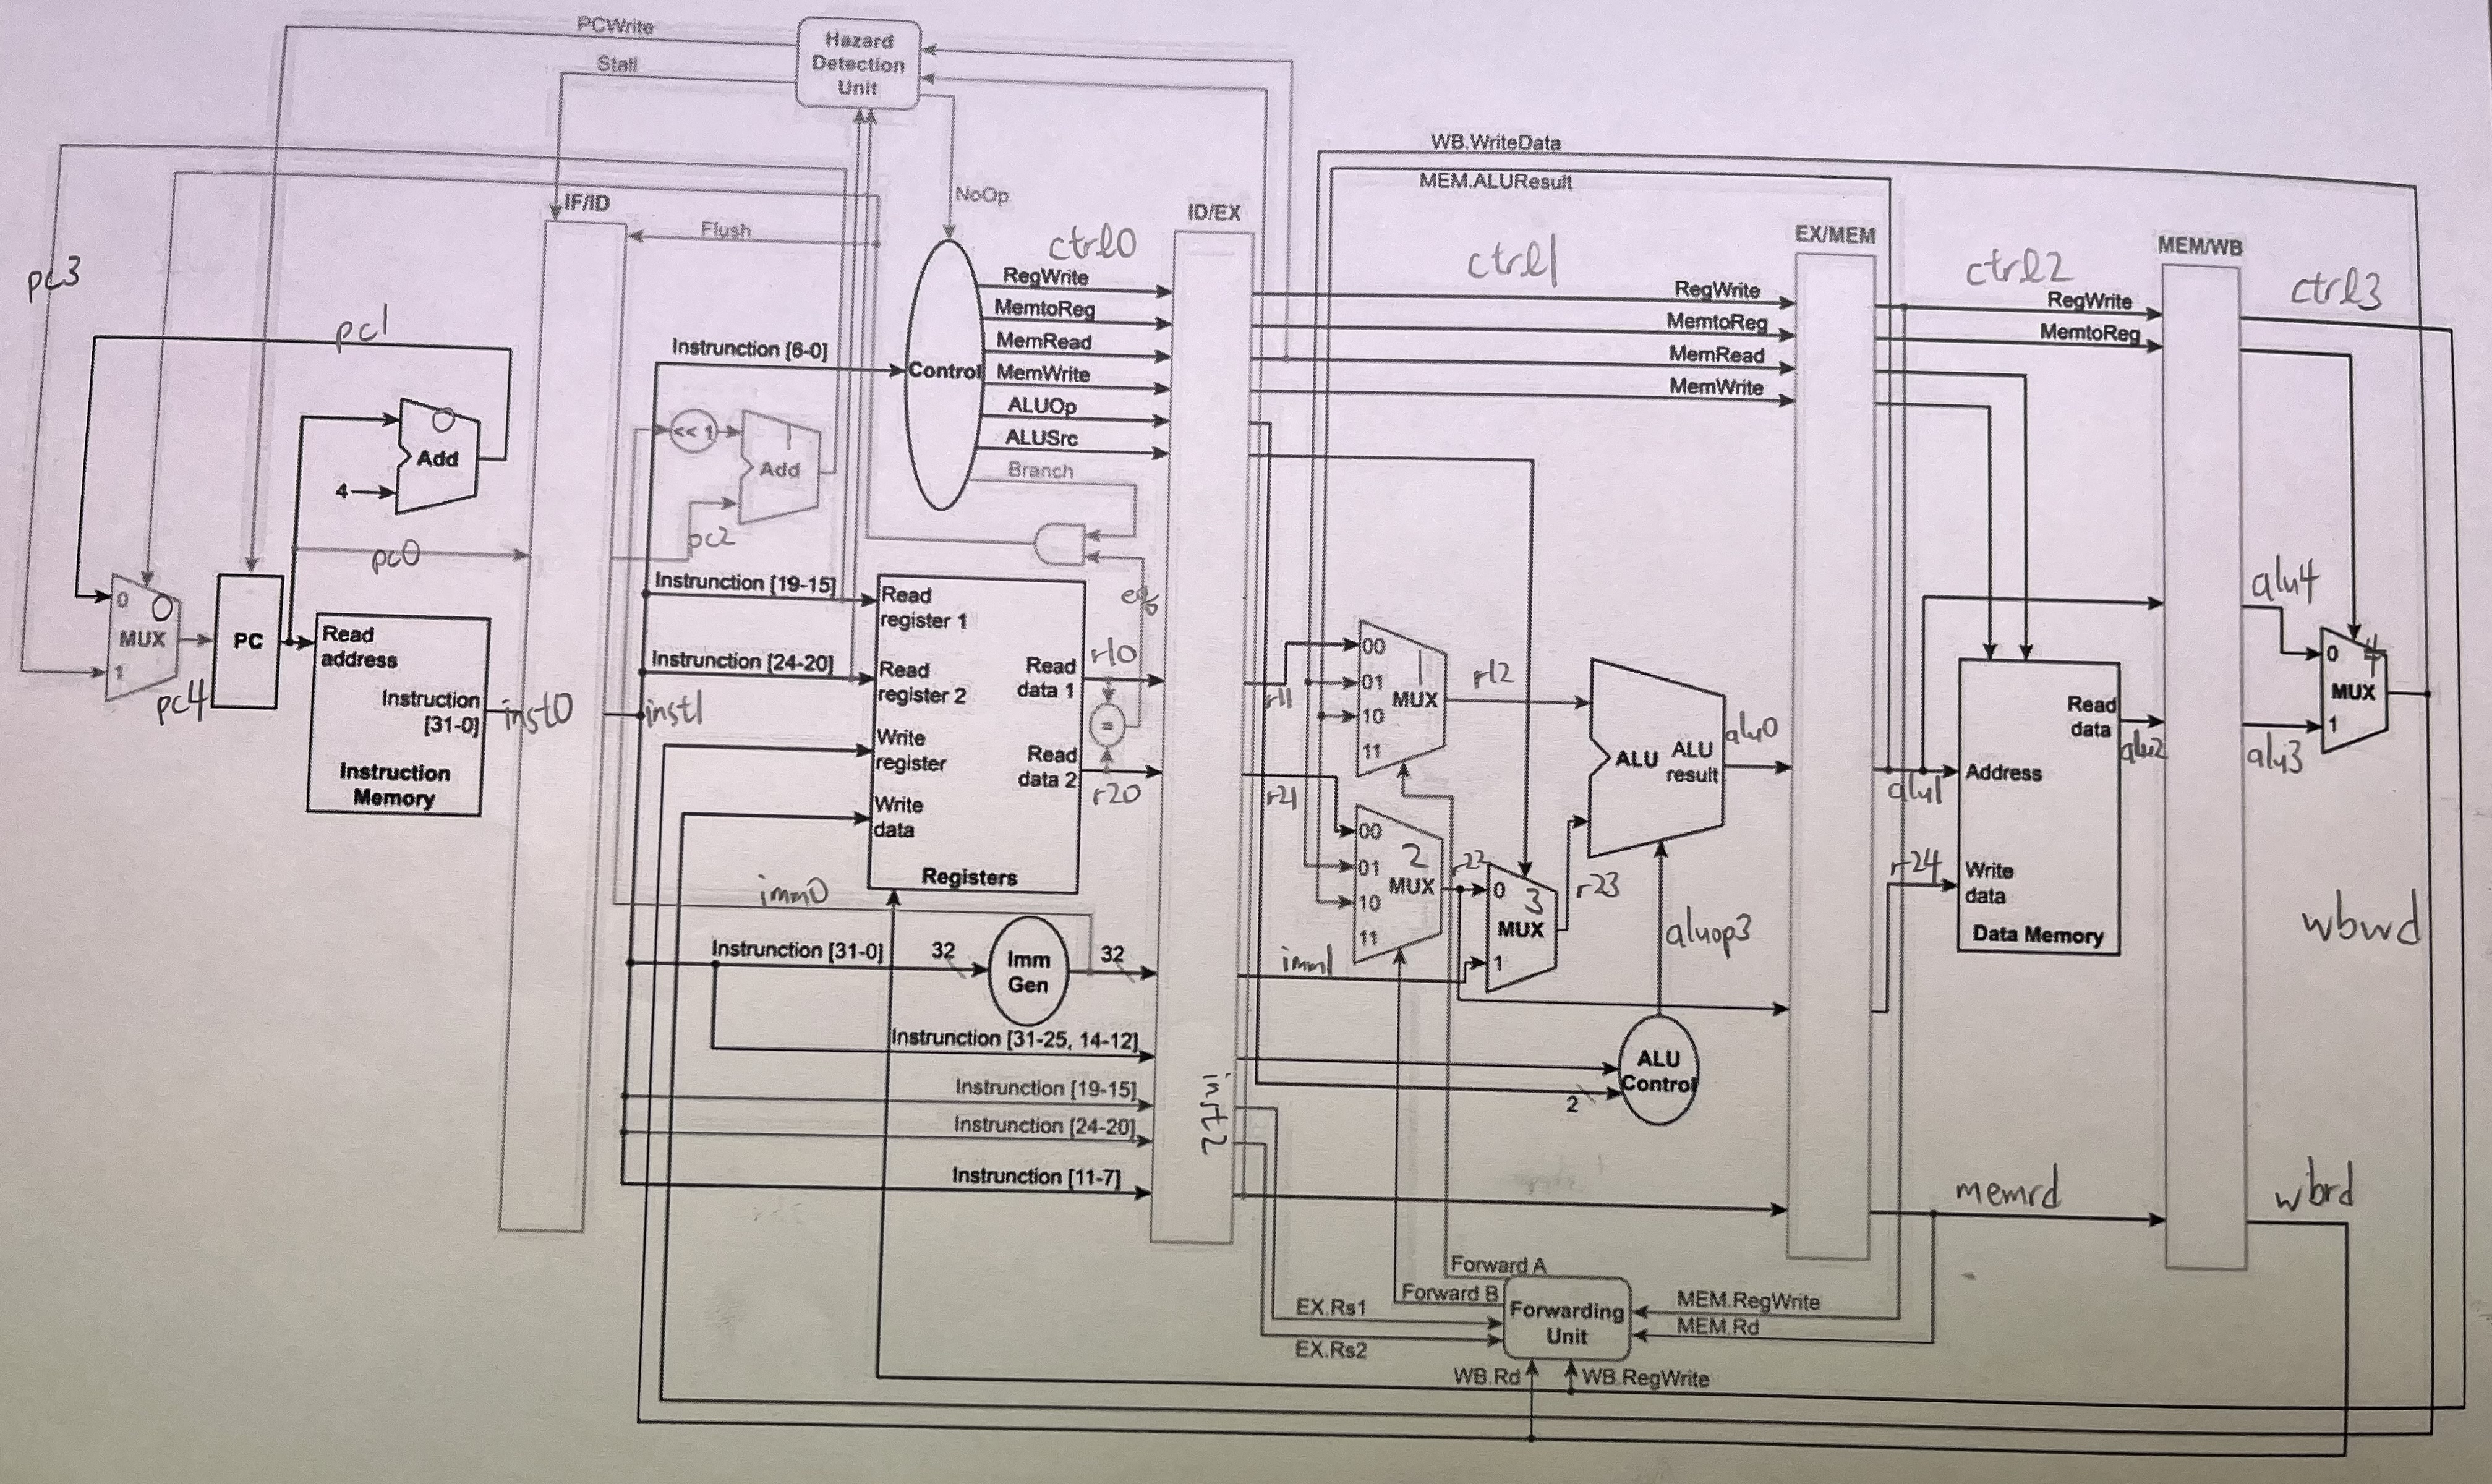
\includegraphics[width=15cm]{all.JPG}\\
where the wires' names are marked above. Note that the wires \texttt{ctrl0}, \texttt{ctrl1}, \texttt{ctrl2}, \texttt{ctrl3} are wires of some control signals (see \texttt{Control, IDEX, EXMEM, MEMWB} modules described above for more detials), the wires \texttt{inst[31..25, 14..12], inst[19..15], inst[24..20], inst[11..7]} at the bottom of the ID stage is replaced by a single wire \texttt{inst1}, and the wires \texttt{inst[31..25, 14..12], inst[19..15], inst[24..20], inst[11..7]} at the bottom of the EX stage is replaced by a single wire \texttt{inst2}.

\section{Difficulties Encountered and Solutions}

When implementing instruction \texttt{beq}, the next instruction after \texttt{beq} shouldn't be done if \texttt{beq} jumped another branch; however, I found that my implementation did since I didn't deal with \texttt{flush} well in \texttt{IFID} module.\\
I used to wonder why \texttt{Control} module needs the \texttt{noop} signal; after reviewing the powerpoints in class again, I found that's because the instruction being done in the ID stage should become bubble.\\
I used to implement all control signals in a single wire, but I found that \texttt{textbench.v} required the wire \texttt{Branch} having the name \texttt{Branch\_o}. Therefore, I changed a lot of modules' implementations including \texttt{Control}, \texttt{IDEX}, \texttt{CPU} modules.

\section{Development Environment}

\begin{itemize}
\item OS: Ubuntu 22.04.2 LTS
\item Compiler: iverilog
\end{itemize}
